\documentclass{article}

\usepackage{amsmath,amssymb}
\usepackage{multicol}
\usepackage{systeme}
\usepackage{url}
%\usepackage{siunitx}

% for drawing graphs
\usepackage{tikz}
\tikzset{every picture/.style={thick}}
\tikzset{every node/.style={draw, circle, inner sep = 2pt}}
\usetikzlibrary{arrows}

% for margins
\usepackage[margin=1in]{geometry}

% for font
\usepackage{euler}
\usepackage[OT1]{eulervm}
\renewcommand{\rmdefault}{pplx}

\setlength{\parindent}{0pt}  %no indenting

% MACROS
\newcommand{\trans}{^\top}
\newcommand{\adj}{^{\rm adj}}
\newcommand{\cof}{^{\rm cof}}
\newcommand{\inp}[2]{\left\langle#1,#2\right\rangle}
\newcommand{\dunion}{\mathbin{\dot\cup}}
\newcommand{\bzero}{\mathbf{0}}
\newcommand{\bone}{\mathbf{1}}
\newcommand{\ba}{\mathbf{a}}
\newcommand{\bb}{\mathbf{b}}
\newcommand{\bd}{\mathbf{d}}
\newcommand{\be}{\mathbf{e}}
\newcommand{\bp}{\mathbf{p}}
\newcommand{\bq}{\mathbf{q}}
\newcommand{\bx}{\mathbf{x}}
\newcommand{\by}{\mathbf{y}}
\newcommand{\bz}{\mathbf{z}}
\newcommand{\bu}{\mathbf{u}}
\newcommand{\bv}{\mathbf{v}}
\newcommand{\bw}{\mathbf{w}}
\newcommand{\tr}{\operatorname{tr}}
\newcommand{\nul}{\operatorname{null}}
\newcommand{\rank}{\operatorname{rank}}
%\newcommand{\ker}{\operatorname{ker}}
\newcommand{\range}{\operatorname{range}}
\newcommand{\Col}{\operatorname{Col}}
\newcommand{\Row}{\operatorname{Row}}
\newcommand{\spec}{\operatorname{spec}}
\newcommand{\vspan}{\operatorname{span}}
% \newenvironment{sol}{\medskip\noindent {\bf Solution.}}{\newpage}
\newcommand{\mystrut}{\rule[-.5\baselineskip]{0pt}{2\baselineskip}}
% \newcommand{\mul}{\operatorname{mul}}
\newcommand{\even}{\operatorname{even}}
\newcommand{\sgn}{\operatorname{sgn}}
\newcommand{\iner}{\operatorname{iner}}
\newcommand{\rL}{\mathring{L}}
\newcommand{\diag}{\operatorname{diag}}

\makeatletter
%%%The definition of \binom is \genfrac ()\z@ {}
%%%To adjust the spaces between parantheses, change the augment of \kern
\newcommand{\multiset}[2]{\ensuremath{\left(\kern-.3em\left(\genfrac{}{}{\z@}{}{#1}{#2}\right)\kern-.3em\right)}}
\newcommand{\qanalog}[2]{\genfrac []\z@ {}{#1}{#2}_q}
\makeatother

% for title
\title{2023F Math585 Midterm 2}
\date{\vspace{-1cm}}
\begin{document}
\maketitle
\large

\textbf{5 questions}, \textbf{$20(+5)$ total points}

\textbf{Note:}  Use other papers to answer the problems.  Remember to write down your \textbf{name} and your \textbf{student ID \#}.

\begin{enumerate}
\setlength\itemsep{2em}

\item{} [5pt] Let $C_n$ be the cycle on $n$ vertices and $A_n$ its adjacency matrix.  For $n\geq 0$, find the $1,1$-entry of $(A_{n+1})^n$.  

\item{} [5pt] Let $G$ be the graphs below and $A$ its adjacency matrix.   Find $\rank(A)$, $\det(A)$, and the inertia of $A$.  
\begin{center}
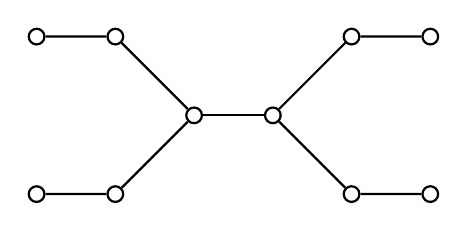
\begin{tikzpicture}
\node (1) at (-2,1) {};
\node (2) at (-1,1) {};
\node (3) at (0,0) {};
\node (4) at (-1,-1) {};
\node (5) at (-2,-1) {};
\node (6) at (3,1) {};
\node (7) at (2,1) {};
\node (8) at (1,0) {};
\node (9) at (2,-1) {};
\node (10) at (3,-1) {};
\draw (1) -- (2) -- (3) -- (4) -- (5);
\draw (6) -- (7) -- (8) -- (9) -- (10);
\draw (3) -- (8);
\end{tikzpicture}
\end{center}


\item{} [5pt] Let  
\[A = \begin{bmatrix}
    0 & 0 & 1 & 1 & 0 & 0 \\
    0 & 0 & 1 & 1 & 0 & 0 \\
    1 & 1 & 0 & 0 & 1 & 1 \\
    1 & 1 & 0 & 0 & 1 & 1 \\
    0 & 0 & 1 & 1 & 0 & 0 \\
    0 & 0 & 1 & 1 & 0 & 0 \\
\end{bmatrix}.
\]
Find $\spec(A)$.  


\vfill

\textbf{Two more problems on the back.}

\newpage
\item{} [5pt] Let $G$ be the graphs below and $A$ its adjacency matrix.  

\begin{center}
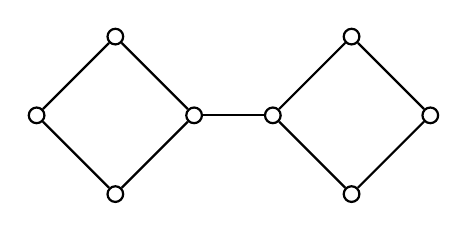
\begin{tikzpicture}
\node (1) at (-2,0) {};
\node (2) at (-1,1) {};
\node (3) at (0,0) {};
\node (4) at (-1,-1) {};
\node (5) at (3,0) {};
\node (6) at (2,1) {};
\node (7) at (1,0) {};
\node (8) at (2,-1) {};
\draw (1) -- (2) -- (3) -- (4) -- (1);
\draw (5) -- (6) -- (7) -- (8) -- (5);
\draw (3) -- (7);
\end{tikzpicture}
\end{center}
Find the characteristic polynomial $\det(A - xI)$ of $A$.

\item{} [extra 5pt] Let 
\[A = \begin{bmatrix}
 O_{m\times m} & B & \\
 C & O_{n\times n} 
\end{bmatrix},\]
where $O$ is the zero matrix of the designated order.  For $\bx\in\mathbb{R}^n$ and $\by\in\mathbb{R}^m$.  Show that $\begin{bmatrix} \bx \\ \by \end{bmatrix}$ is an eigenvector of $A$ with respect to $\lambda$ if and only if $\begin{bmatrix} \bx \\ -\by \end{bmatrix}$ is an eigenvector of $A$ with respect to $-\lambda$.
\end{enumerate}

\end{document}



  
